\chapter{System Requirements and Architecture}

\section{Introduction}

OrchardVision is a full-stack system consisting of a FastAPI backend, a React~+~TypeScript frontend and a set of core services that implement the computer vision pipeline. This chapter states the requirements that the system satisfies and describes its architecture and technology stack.

\section{Requirements}

\subsection{Functional Requirements}

\add{The functional requirements below were derived from the capabilities of the implemented system:}

\begin{itemize}
  \item \add{FR1: upload a video, store it, and extract its metadata (width, height, frame rate and frame count).}
  \item \add{FR2: start, monitor and complete a processing job for an uploaded video, and reject a new job while another is active.}
  \item \add{FR3: persist tracks, detections, identities, ReID events, camera-motion estimates and per-frame timing for each processed video.}
  \item \add{FR4: retrieve every persisted artefact through the REST API, including a two-dimensional projection of identity prototypes.}
  \item \add{FR5: create, run, list, export and delete evaluation experiments for different trackers and scenarios.}
  \item \add{FR6: read and update the default pipeline settings.}
  \item \add{FR7: delete a video together with all associated data.}
\end{itemize}

\subsection{Non-Functional Requirements}

\begin{itemize}
  \item \add{\textbf{Portability.} The same code runs on a developer laptop and in the container stack; because all persistence goes through the SQLAlchemy ORM, the database is selected purely by the connection string in \code{DATABASE_URL}}.
  \item \add{\textbf{Responsiveness.} Long-running processing must not block API requests; it is executed as a background task or through a Celery queue.}
  \item \add{\textbf{Consistency.} All errors use a single JSON structure and the frontend and backend share type definitions.}
  \item \add{\textbf{Extensibility.} New models, routers, schemas and services can be added in separate modules without modifying existing ones.}
  \item \add{\textbf{Isolation of binary data.} Videos and cached frames are written to the file system through the storage service rather than into the database, so large payloads never travel through SQL.}
\end{itemize}

\section{High-Level Architecture}

Figure~\ref{fig:arch} shows the components of OrchardVision and their interaction. The React client talks to the FastAPI backend over REST under the \code{/api} prefix; the backend uses the core services to process videos, persists results through SQLAlchemy and writes binary data to the file system.

\begin{figure}[htbp]
\centering
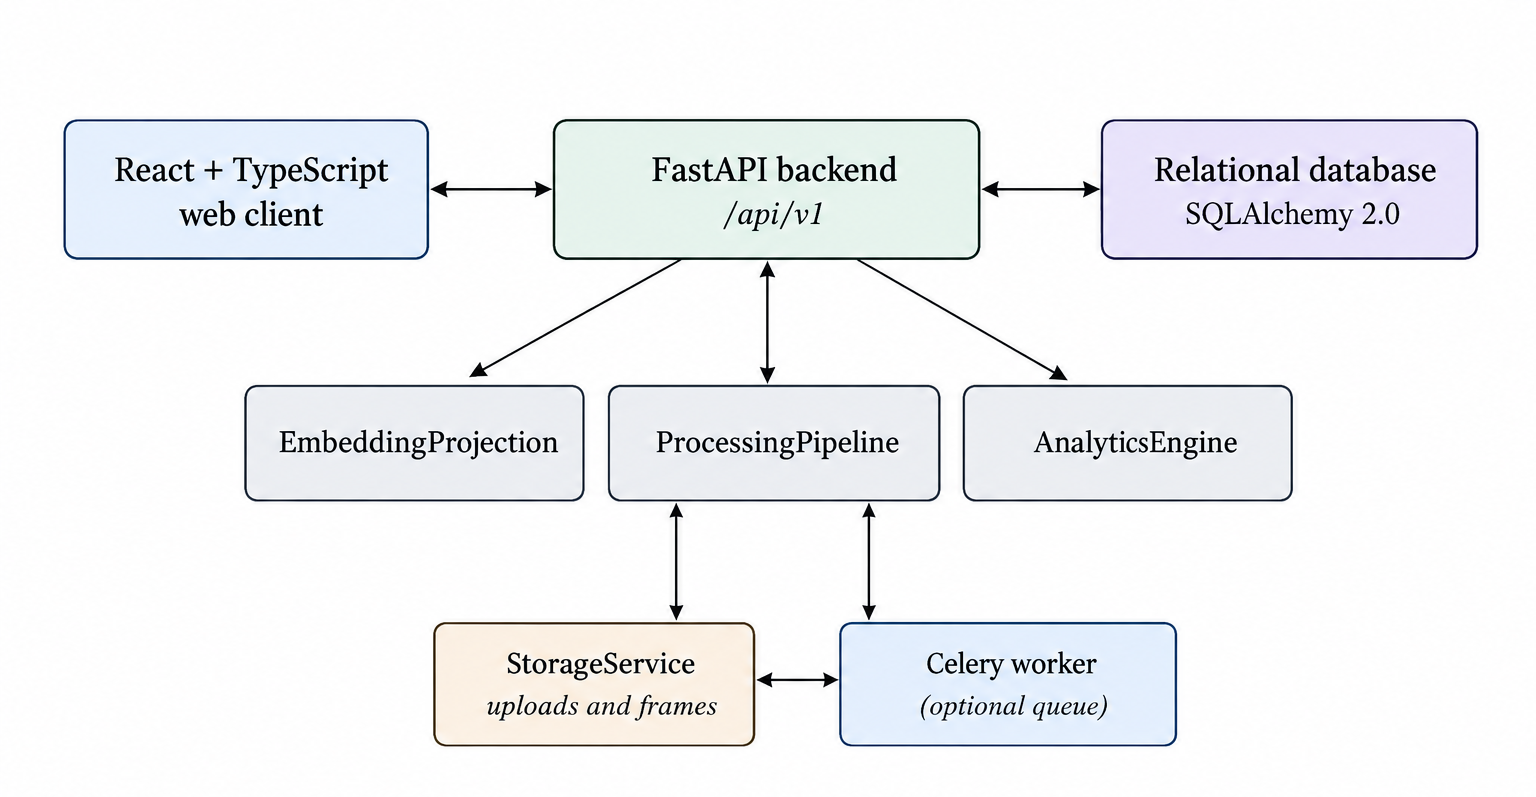
\includegraphics[width=0.95\linewidth]{architecture.png}
\caption[High-level architecture of OrchardVision]{High-level architecture of OrchardVision showing the web client, FastAPI backend, core services, relational database, file storage and optional Celery worker.}
\label{fig:arch}
\end{figure}

\section{Backend}

The backend is implemented with the following choices:

\begin{itemize}
  \item \textbf{Framework:} FastAPI with the SQLAlchemy~2.0 ORM.
  \item \textbf{Database:} SQLite, selected through the \code{DATABASE_URL} environment variable; the ORM layer allows a server database to be substituted without code changes.
  \item \textbf{API:} REST under \code{/api/v1/}, organised in router prefixes for health (\code{GET /health}), videos (\code{POST/GET/DELETE /videos}), tracks (\code{GET /videos/{id}/tracks}), identities (\code{GET /videos/{id}/identities}), processing (\code{POST /videos/{id}/process}), jobs (\code{GET /jobs/{id}}), experiments (\code{GET/POST/DELETE /experiments}) and settings (\code{GET/PUT /settings}).
\end{itemize}

\section{Frontend}

The frontend is a React and TypeScript application. Types shared with the API are defined once in \code{packages/types/src/}, the components live in \code{apps/web/src/}, and an API client calls the FastAPI backend. During development the Vite server proxies requests under \code{/api/} to the backend.

\section{Core Services}

\begin{itemize}
  \item \textbf{ProcessingPipeline.} Orchestrates frame extraction $\rightarrow$ detection $\rightarrow$ tracking $\rightarrow$ embedding $\rightarrow$ analytics.
  \item \textbf{EmbeddingProjection.} Produces t-SNE / PCA visualisations of identity prototypes, served as two-dimensional coordinates.
  \item \textbf{AnalyticsEngine.} Computes IDF1, HOTA and ID-switch metrics.
  \item \textbf{StorageService.} Saves uploads under \code{UPLOAD_DIR} and renders cached JPEG frames under \code{UPLOAD_DIR/frames/<video\_id>}, validating that resolved paths stay inside the upload directory.
\end{itemize}

\section{Configuration}

Configuration is loaded through \code{pydantic_settings} from an \code{.env} file. The key settings are the confidence threshold, the ReID threshold, the tracker type, the camera-motion mode, the memory update rate, the tracker match threshold and the number of buffer frames. The defaults are persisted in the \code{AppSettings} table, which holds a single row identified by \code{GLOBAL_SETTINGS_ID}, and can be read and updated through \code{GET /settings} and \code{PUT /settings}.

\section{Actors and Use Cases}

\add{Two kinds of users interact with the system. An \emph{analyst} (for example an agronomist or a student researcher) uploads videos, starts processing, inspects tracks and identities and reads analytics. An \emph{experimenter} additionally creates and compares experiments and edits the pipeline defaults. The main use cases are: upload video, process video, view tracks, view identities and their projection, view ReID events, view analytics, manage experiments, export results, edit settings and delete video.}

\figph{fig:usecase}{Use-case diagram}{Use-case diagram of OrchardVision.}{UML use-case diagram. Two actors on the left (Analyst, Experimenter) and the system boundary ``OrchardVision'' containing the ten use cases listed above. Draw Experimenter as a specialisation of Analyst, and connect ``Process video'' with an \texttt{include} relationship to ``Upload video''.}{6cm}

\section{Hardware and Software Requirements}

\begin{table}[htbp]
\centering\small
\begin{tabular}{@{}>{\raggedright\arraybackslash}p{3.6cm}>{\raggedright\arraybackslash}p{10.2cm}@{}}
\toprule
\hr \textbf{Item} & \textbf{Requirement}\\
\midrule
\hr Operating system & Linux, macOS or Windows capable of running Python, Node.js and Docker\\
\hr Python & Python environment with FastAPI, SQLAlchemy 2.0, pydantic-settings, uvicorn, Celery, OpenCV and the detection/tracking libraries used by the pipeline\\
\hr Node.js & Node.js with npm and pnpm for the frontend and the shared types package\\
\hr Database & SQLite\\
\hr File storage & Local disk through the storage service\\
\hr Compute & \pp{CPU / GPU model and memory used for the experiments}\\
\hr Browser & A current desktop browser (the frontend is served by Vite in development)\\
\bottomrule
\end{tabular}
\caption[Hardware and software requirements]{\add{Hardware and software requirements.}}
\label{tab:reqs}
\end{table}

\section{Technology Stack}

\begin{table}[htbp]
\centering\small
\begin{tabular}{@{}p{4.2cm}p{9.6cm}@{}}
\toprule
\textbf{Layer} & \textbf{Technology}\\
\midrule
Web framework & FastAPI served by uvicorn (gunicorn/uvicorn in production)\\
ORM / database & SQLAlchemy 2.0; SQLite (substitutable through \code{DATABASE_URL})\\
Settings & \code{pydantic_settings} loading \code{.env}\\
Background work & FastAPI background task, or Celery when a queue is configured\\
File storage & Local disk (uploads and frame cache)\\
Frontend & React, TypeScript, Vite\\
Shared contracts & TypeScript package in \code{packages/types/src/}\\
Testing / checks & \code{pytest}; \code{pnpm exec tsc --noEmit}\\
\bottomrule
\end{tabular}
\caption{Technology stack of OrchardVision.}
\label{tab:stack}
\end{table}

\section{Repository Organisation}

New models and migrations are added as SQLAlchemy~2.0 model definitions. New API routes live in \code{apps/api/app/routers/}, schemas in \code{apps/api/app/schemas/} and services in \code{apps/api/app/services/}. The application entry point and the global exception handler are in \code{apps/api/app/main.py}. The complete layout is given in Appendix~A.
